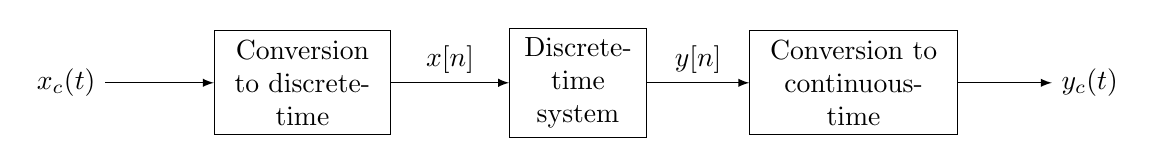
\begin{tikzpicture}
	\node (a) at (0,0) { $x_c(t)$};
	\path (a) -- ++(3,0) node[text width=2cm, draw, align=center] (b) {Conversion to discrete-time}  -- ++(3.5,0) node[text width=1.5cm, draw, align=center] (c) {Discrete-time system}  -- ++(3.5,0) node[text width=2.4cm, draw, align=center] (d) {Conversion to continuous-time}  -- ++(3,0) node (e) { $y_c(t)$};
	\draw[-latex] (a) edge (b);
	\draw[-latex] (b) edge  node[above] {$x[n]$}(c);
	\draw[-latex] (c) edge  node[above] {$y[n]$}(d);
	\draw[-latex] (d) edge  (e);
\end{tikzpicture} 